\documentclass[11pt]{article}
\usepackage[utf8]{inputenc}
\usepackage{amsmath}
\usepackage{amssymb}
\usepackage{graphicx}
\usepackage{hyperref}
\usepackage[parfill]{parskip}
\let\oldemptyset\emptyset
\let\emptyset\varnothing


\title{\textbf{Esssentials of Applied Data Analysis\\
				IPSA-USP Summer School 2017}\newline\\
				Continous Random Variables}

\author{Leonardo Sangali Barone\\ \href{leonardo.barone@usp.br}{leonardo.barone@usp.br}}
\date{jan/17}

\begin{document}

\maketitle

\section*{Continuous random variables}
	
	The rules that apply to discrete random variables also apply to continous random variables.\\
	
	The main problem when we deal with a continuous random variable is that we cannot count every possible outcome and multiply it by the probability of that outcome occurin (remember: continous variables are and infinite set and uncontable!)\\

\subsection*{A very bad example from Fakeland}

If we tried to tabulate a continious variable, for example, income, our table would be like this:

\begin{tabular}{|c|c|c|c|}
\hline
$x_i$	&	f$(x_i)$	&	$x_i$	&	f$(x_i)$	\\
\hline
$43,69$	&	$1/30$	&	$2724,15$	&	$1/30$	\\
$266,92$	&	$1/30$	&	$2826,06$	&	$1/30$	\\
$448,05$	&	$1/30$	&	$2879,75$	&	$1/30$	\\
$508,59$	&	$1/30$	&	$2929,64$	&	$1/30$	\\
$524,24$	&	$1/30$	&	$3017,94$	&	$1/30$	\\
$652,70$	&	$1/30$	&	$4035,14$	&	$1/30$	\\
$874,76$	&	$1/30$	&	$4072,06$	&	$1/30$	\\
$1407,38$	&	$1/30$	&	$4180,46$	&	$1/30$	\\
$2108,53$	&	$1/30$	&	$4537,20$	&	$1/30$	\\
$2166,74$	&	$1/30$	&	$4619,97$	&	$1/30$	\\
$2202,34$	&	$1/30$	&	$6404,45$	&	$1/30$	\\
$2219,01$	&	$1/30$	&	$6463,01$	&	$1/30$	\\
$2300,42$	&	$1/30$	&	$6540,19$	&	$1/30$	\\
$2595,25$	&	$1/30$	&	$6696,28$	&	$1/30$	\\
$2686,48$	&	$1/30$	&	$8213,81$	&	$1/30$	\\
\hline
\end{tabular}

Not very interesting, is it?\\

Well, we could aggregate values into value ranges. For example, we could recode our variable into a new one that contain only two values, ``$\$ 3,000.00 \text{ or less}$'' ``$\text{more than }\$ 3,000.00$''. It would be fine, but we would loose information (variation within the category) of our variable.\\

Continuous random variables are better displayed graphically. In particular, histograms and density plots are a good choice. See Figure~\ref{f1}\\

\begin{figure}[htp]
\centering
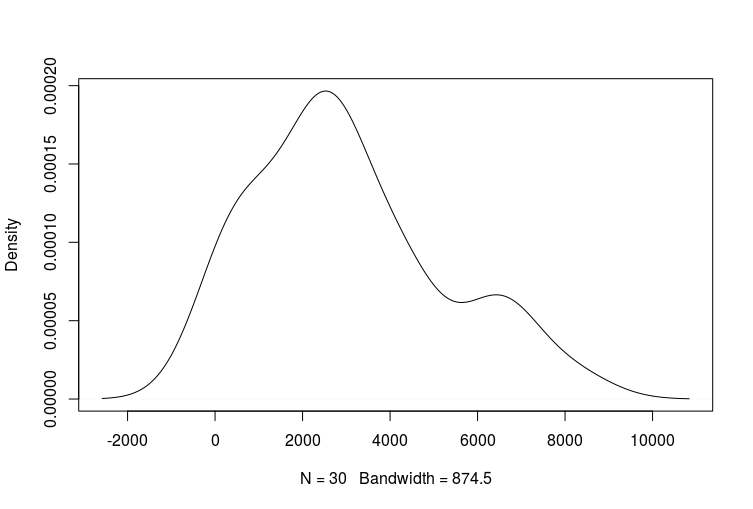
\includegraphics[scale=0.60]{income_density.png}
\caption{Income Distribution in Fakeland - sample data}
\label{f1}
\end{figure}

In one of the next handouts we are going to work with HDI (Human Develepment Index) Data for Brazilian municipailities. There are 5565 municipailities and most of them have unique values for the index. Again, it makes a lot more sense to exam the data graphically than with tables. Check Figure~\ref{f2}

\begin{figure}[htp]
\centering
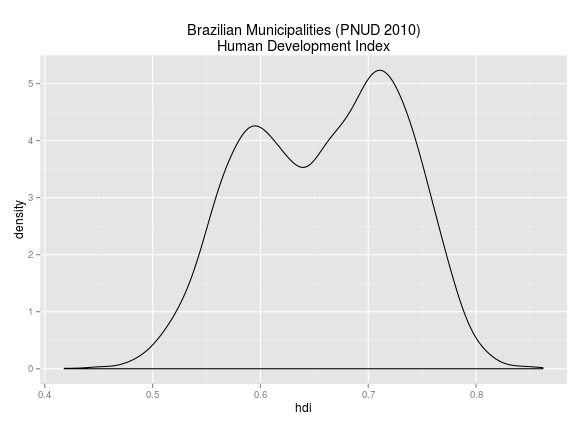
\includegraphics[scale=0.60]{clt_pop_dist.png}
\caption{}
\label{f2}
\end{figure}

\end{document}
